\subsection*{Problema 03}
Evaluar la integral definida mediante sumas de Riemann:
\begin{align*}
    I = \int_{1}^{2} x \, dx
\end{align*}

\textbf{Solución:}
Dividimos el intervalo $[1, 2]$ en $n$ subintervalos iguales de ancho:
\begin{align*}
    \Delta x = \dfrac{2 - 1}{n} = \dfrac{1}{n}
\end{align*}

Los puntos extremos derechos de cada subintervalo se definen como:
\begin{align*}
    x_i = 1 + i \Delta x = 1 + \dfrac{i}{n}, \quad i = 1, 2, \dots, n
\end{align*}

Planteamos la suma de Riemann usando el límite cuando $n \to \infty$:
\begin{align*}
    I &= \lim_{n \to \infty} \sum_{i=1}^{n} f(x_i) \Delta x \\
    I &= \lim_{n \to \infty} \sum_{i=1}^{n} \left(1 + \dfrac{i}{n}\right) \dfrac{1}{n}
\end{align*}

Extraemos las constantes y distribuimos la sumatoria:
\begin{align*}
    I &= \lim_{n \to \infty} \dfrac{1}{n} \left[ \sum_{i=1}^{n} 1 + \dfrac{1}{n} \sum_{i=1}^{n} i \right]
\end{align*}

Aplicamos las fórmulas para $\sum 1 = n$ y $\sum i = \dfrac{n(n+1)}{2}$:
\begin{align*}
    I &= \lim_{n \to \infty} \dfrac{1}{n} \left[ n + \dfrac{n(n+1)}{2n} \right] \\
    I &= \lim_{n \to \infty} \left[ 1 + \dfrac{n+1}{2n} \right]
\end{align*}

Simplificamos el límite algebraicamente:
\begin{align*}
    I &= \lim_{n \to \infty} \left( 1 + \dfrac{1}{2} + \dfrac{1}{2n} \right) \\
    I &= 1 + \dfrac{1}{2} + 0 = \dfrac{3}{2}
\end{align*}

El valor exacto de la integral es $1.5$.

\begin{figure}[H]
	\centering
	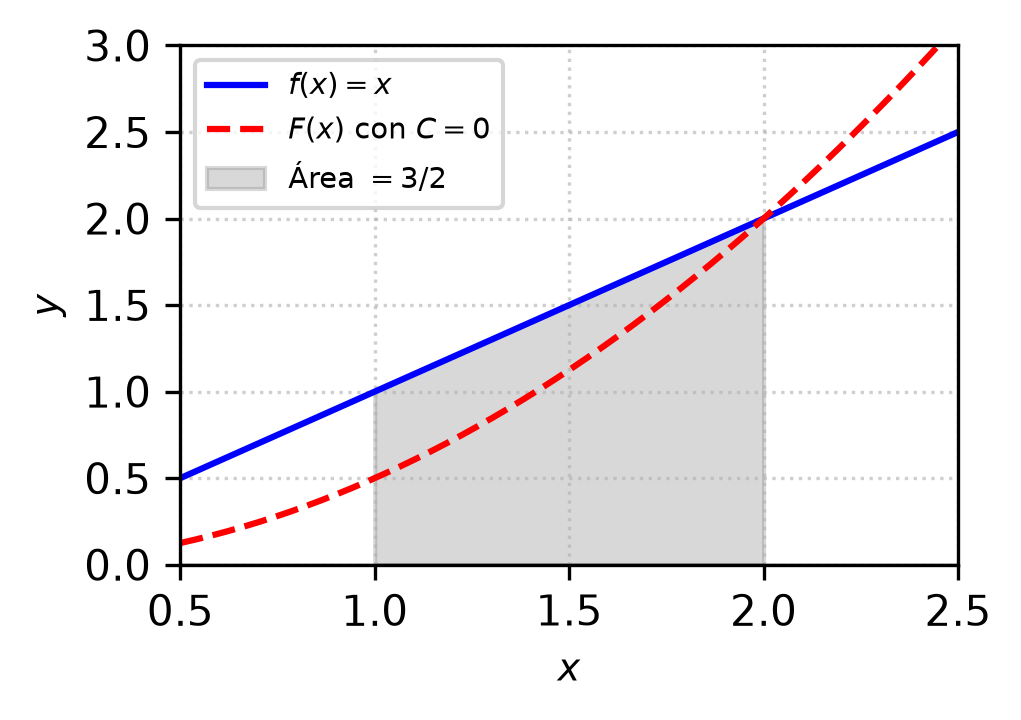
\includegraphics[width=\columnwidth]{semana_06/graficas/SEM06_P03_grafica.png}
	\caption{Representación gráfica de $f(x)$ y su antiderivada $F(x)$ evaluada para la constante de integración $C = 0$ (Problema 03).}
	\label{fig:problema03}
\end{figure}
